\documentclass[twoside,final]{hcmut-report}

\usepackage[utf8]{inputenc}
\usepackage[T5]{fontenc}
\usepackage[vietnamese]{babel}
% \usepackage{vntex}
\usepackage[protrusion=false]{microtype}

\usepackage{graphicx, caption}
\usepackage{amsmath}
\usepackage{xcolor}
\usepackage{listings}
\usepackage{multirow,multicol}
\usepackage{enumitem}
\usepackage{hyperref}
\usepackage{float}
\usepackage{booktabs}
\usepackage{longtable}
\usepackage{array}
\usepackage{tabularx}
\usepackage{makecell}
\usepackage{subcaption}
\usepackage{tikz}
\usepackage{pgfplots}
\usepackage[most]{tcolorbox}
\usepackage{wrapfig}

\AtBeginDocument{\counterwithin{lstlisting}{section}}
\newtcolorbox{exercisebox}{
  enhanced,
  breakable,
  colback=white,
  colframe=black,
  arc=3mm,
  boxrule=0.4pt,
  width=\textwidth,
  left=5pt,
  right=5pt,
  top=5pt,
  bottom=5pt,
  fontupper=\normalsize,
  before upper={\setlength{\parindent}{2em}}
}
\newcommand{\exercise}[1]{\begin{exercisebox}#1\end{exercisebox}}
\begin{document}

\coverpage\clearpage
\tableofcontents
\clearpage

\fancyfoot{}
\fancyfoot[L]{\scriptsize \ttfamily Toán 12 - Ltro x doxncwfn - 2526}
\fancyfoot[R]{\scriptsize \ttfamily Trang {\thepage}/\pageref{LastPage}}

\setcounter{page}{1}
\section{Xác suất thống kê}
\subsection{Lý thuyết}
\subsection{Định nghĩa}
Cho hai biến cố $A$ và $B$. Xác suất của biến cố $A$ với điều kiện biến cố $B$ đã xảy ra được gọi là xác suất của $A$ với điều kiện $B$, kí hiệu là $P(A | B)$.

Nếu $P(B) > 0$ thì:
\[
    P(A | B) = \frac{P(A \cap B)}{P(B)}.
\]
\paragraph*{Nhận xét}
\begin{itemize}[itemsep=0pt, topsep=0pt, parsep=0pt,label=-]
    \item Từ định nghĩa của xác suất có điều kiện, ta suy ra $P(A \cap B) = P(B) \cdot P(A | B)$.
    \item Người ta chứng minh được rằng
          \[
              \mathrm{P}(A \cap B) = \mathrm{P}(A) \cdot \mathrm{P}(B | A) = \mathrm{P}(B) \cdot \mathrm{P}(A | B).
          \]
          Công thức trên được gọi là \textbf{công thức nhân xác suất}.
    \item Người ta cũng tính $P(A | B) = \dfrac{n(A \cap B)}{n(B)}$.
\end{itemize}
\subsubsection{Công thức xác suất đầy đủ}
Cho 2 biến cố $A$, $B$ với $0 < P(B) < 1$, ta có:
\[
    P(A) = P(A \cap B) + P(A \cap \overline{B}).
\]

Mặt khác:
\begin{align*}
    P(A \cap B)            & = P(B) \cdot P(A | B)                       \\
    P(A \cap \overline{B}) & = P(\overline{B}) \cdot P(A | \overline{B})
\end{align*}

Từ đó ta có công thức xác suất đầy đủ như sau:
\[
    P(A) = P(B) \cdot P(A | B) + P(\overline{B}) \cdot P(A | \overline{B}).
\]
\subsubsection{Công thức Bayes}
Từ công thức nhân xác suất:
\[
    P(B | A) \cdot P(A) = P(B) \cdot P(A | B) = P(A \cap B).
\]

Với hai biến cố $A, B$ mà $P(A) > 0$, ta có công thức xác suất Bayes:
\[
    P(B | A) = \frac{P(B) \cdot P(A | B)}{P(A)}.
\]

Do \(P(A) = P(B) \cdot P(A | B) + P(\overline{B}) \cdot P(A | \overline{B})\), nên công thức Bayes còn có dạng:
\[
    P(B | A) = \frac{P(B) \cdot P(A | B)}{P(B) \cdot P(A | B) + P(\overline{B}) \cdot P(A | \overline{B})}.
\]
\subsection{Bài tập}
\exercise{Theo một số liệu thống kê, năm 2004 ở Canada có 65\% nam giới là thừa cân và 53,4\% nữ giới là thừa cân. Nam giới và nữ giới ở Canada đều chiếm 50\% dân số cả nước. Hỏi trong năm 2004, xác suất để một người Canada được chọn ngẫu nhiên là người thừa cân bằng bao nhiêu?}

Xét hai biến cố:
\begin{itemize}[itemsep=0pt, topsep=0pt, parsep=0pt,label=-]
    \item $A$: ``Người được chọn ra là người thừa cân'';
    \item $B$: ``Người được chọn ra là nam giới'' $\Rightarrow\overline{B}$: ``Người được chọn ra là nữ giới''.
\end{itemize}

Từ giả thiết:
$\begin{cases}
        \mathrm{P}(B) = \mathrm{P}(\overline{B}) = 50\% = 0{,}5 \\
        \mathrm{P}(A | B) = 65\% = 0{,}65                       \\
        \mathrm{P}(A | \overline{B}) = 53{,}4\% = 0{,}534.
    \end{cases}$

Theo công thức xác suất toàn phần:
\[
    \mathrm{P}(A) = \mathrm{P}(B) \cdot \mathrm{P}(A | B) + \mathrm{P}(\overline{B}) \cdot \mathrm{P}(A | \overline{B})
    = 0{,}5 \cdot 0{,}65 + 0{,}5 \cdot 0{,}534 = 0{,}592.
\]
\subsection{Đề thi thử trường sở}
\exercise{\textcolor{red}{\textit{Đợt 3 -- 2425 -- Nghệ An}}

    \begin{wrapfigure}{r}{0.17\textwidth}
        \centering
        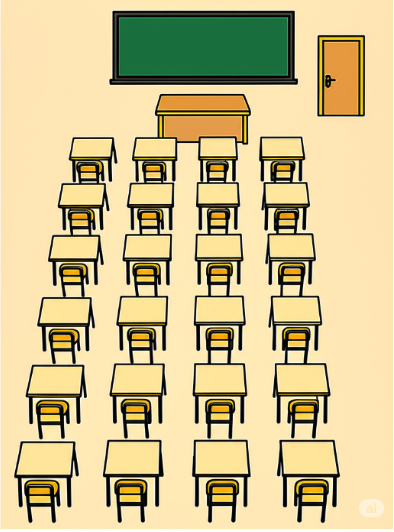
\includegraphics[width=1.08\linewidth]{images/Nghệ An 2025 - Đợt 3/NgheAn25-2.png}
    \end{wrapfigure}
    Cúm A (Influenza A) là bệnh nhiễm trùng đường hô hấp cấp tính do các virus cúm mùa gây nên. Virus cúm A có thể lây truyền trực tiếp trong không khí thông qua đường hô hấp. Giả sử Virut cúm A có khả năng lấy nhiễm đối với người ngồi trong vòng bán kính $1,9m$ là $85\%$ và đối với người ngồi cách hơn $1,9m$ là $5\%$. An là một học sinh bị nhiễm cúm A nhưng bản thân không hay biết. An đi dự thi cuối kỳ. Phòng thi của An có $24$ bạn được xếp vào $24$ chỗ ngồi của một phòng thi có $4$ dãy, mỗi dãy $6$ chỗ ngồi như hình vẽ. Khoảng cách giữa hai người theo hàng ngang là $1,6m$, theo hàng dọc là 1m (hình vẽ). Do không biết trước An bị cúm A nên các thí sinh được xếp ngẫu nhiên vào phòng thi. Một bạn cùng phòng của An sau khi dự thi đi kiểm tra thấy không bị nhiễm cúm. Tính xác suất để thí sinh đó ngồi gần An trong vòng $1,9m$. \textit{(Làm tròn kết quả đến hàng phần trăm)}.
}
\begin{wrapfigure}{l}{0.25\textwidth}
    \centering
    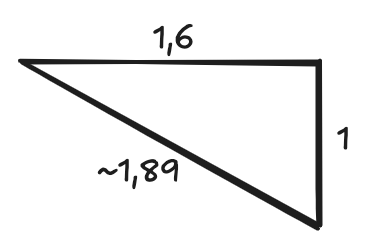
\includegraphics[width=0.8\linewidth]{images/Nghệ An 2025 - Đợt 3/NgheAn25-3.png}
    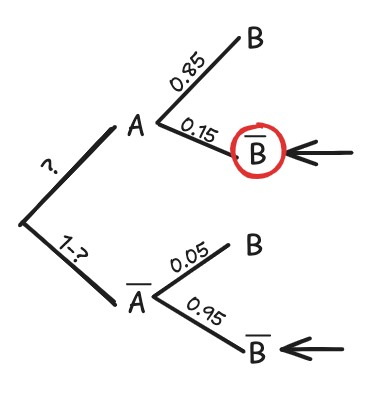
\includegraphics[width=1.2\linewidth]{images/Nghệ An 2025 - Đợt 3/NgheAn25-4.png}
\end{wrapfigure}
Gọi $A$ là biến cố ngồi gần An, $B$ là biến cố bị nhiễm bệnh.\\
Vì nếu ngồi chéo An thì bạn đó vẫn bị nhiễm bệnh nên xét vị trí An được xếp:
\begin{itemize}[itemsep=0pt, topsep=0pt, parsep=0pt,label=-]
    \item Nếu An ngồi ở 1 trong 4 góc phòng, chỉ có $3$ vị trí trong bán kính lây bệnh.
    \item Nếu An ngồi ở 1 trong 12 rìa phòng, có $5$ vị trí trong bán kính lây bệnh.
    \item Nếu An ngồi ở 1 trong 8 vị trí giữa phòng, có $8$ vị trí trong bán kính lây bệnh.
\end{itemize}

$\Rightarrow P(A) = \dfrac{4}{24}\cdot\dfrac{3}{23} + \dfrac{12}{24}\cdot\dfrac{5}{23} + \dfrac{1}{8}\cdot\dfrac{8}{23} = \dfrac{17}{69} \Rightarrow P(\overline{A}) = \dfrac{52}{69}$\\
$\Rightarrow P(A|\overline{B}) = \dfrac{\dfrac{17}{69}\cdot 0.15}{\dfrac{17}{69}\cdot 0.15 + \dfrac{52}{69}\cdot0.95} \approx 0.0491 \approx 0.05$

\exercise{\textcolor{orange}{\textit{Đợt 3 -- 2425 -- Nghệ An}}

    Một nghiên cứu dịch tễ học trong một cộng đồng dân số tại một địa phương X đưa ra các số liệu sau:
    \begin{itemize}[itemsep=0pt, topsep=0pt, parsep=0pt,label=-]
        \item Tỷ lệ người có hút thuốc lá là 25\%.
        \item Tỷ lệ bị ung thư phổi ở nhóm người hút thuốc lá là 2\%, trong khi ở nhóm người không hút thuốc lá chỉ là 0,1\%.
    \end{itemize}

    Xét một người được chọn ngẫu nhiên từ cộng đồng này. Ký hiệu $A$ là biến cố "Người đó bị ung thư phổi" và $B$ là biến cố "Người đó có hút thuốc lá".
    \begin{enumerate}[itemsep=0pt, topsep=0pt, parsep=0pt,label=\alph*)]
        \item $P(A|B) = 0,1$
        \item Nếu một người bị ung thư phổi, thì xác suất người đó có hút thuốc lá là 0,8 (làm tròn đến hàng phần mười).
        \item Tỷ lệ người bị ung thư phổi ở địa phương X là 1,5\%
        \item Dựa trên các số liệu này, tỷ lệ người bị ung thư phổi ở nhóm người có hút thuốc lá cao gấp 20 lần so với ở nhóm người không hút thuốc.
    \end{enumerate}}
\begin{minipage}{0.55\textwidth}
    a) Từ đề bài: $\begin{cases}
            P(A|B)=2\%                \\
            P(A|\overline{B}) = 0,1\% \\
            P(B) = 0.25
        \end{cases} \Rightarrow$ \textcolor{red}{Sai}\\

    b) $P(A|B) = \dfrac{2\%\cdot 0.25}{2\%\cdot 0.25 + 0.75\cdot 0.1\%} = \dfrac{20}{23} \approx 0.9 \Rightarrow$ \textcolor{red}{Sai}\\

    c) $P(A) = 2\%\cdot 0.25 + 0.1\%\cdot 0.75 = 5.75\%\Rightarrow$ \textcolor{red}{Sai}\\

    d) $\dfrac{P(A|B)}{P(A|\overline{B})} = \dfrac{2\%}{0.1\%} = 20\Rightarrow$  \textcolor{red}{Đúng}
\end{minipage}
\begin{minipage}{0.4\textwidth}
    \begin{figure}[H]
        \centering
        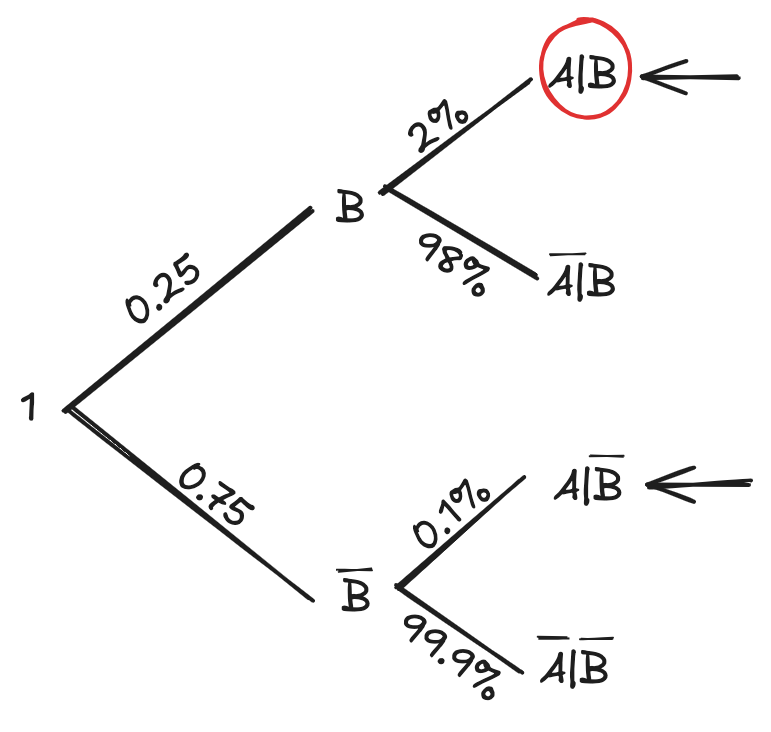
\includegraphics[width=\textwidth]{images/Nghệ An 2025 - Đợt 3/NgheAn25-1.png}
    \end{figure}
\end{minipage}
\section{Ứng dụng tích phân}
\exercise{
    \textcolor{red}{\textit{Đợt 3 -- 2425 -- Nghệ An}}

    \begin{wrapfigure}{r}{0.35\textwidth}
        \centering
        \includegraphics*[width=0.3\textwidth]{images/Nghệ An 2025 - Đợt 3/NgheAn25-5.png}
    \end{wrapfigure}

    Một lập trình viên tạo một trò chơi. Trong trò chơi đó có một vùng đất hình chữ nhật $ABCD$. Một con sông nằm bên cạnh vùng đất đó, $AD$ là bờ sông. Một giếng nước khoan được đặt tại điểm $I$ nằm trong hình chữ nhật, với:
    $AB = 80$m, $AD = 40$m. Điểm $I$ cách cạnh $AB$ $20$m, cách cạnh $AD$ $60$m. Nhân vật trong game khi đến vùng đất này cần phải di chuyển đến giếng nước hoặc bờ sông để lấy nước.

    Lập trình viên muốn tô màu một phần của vùng đất đó sao cho khi đứng trong vùng tô màu này, nhân vật di chuyển đến giếng nước để lấy nước nhanh hơn so với đến bờ sông.

    Diện tích vùng tô màu đó là bao nhiêu mét vuông? (Giả sử rằng khi di chuyển, vận tốc của nhân vật không đổi; làm tròn kết quả đến hàng đơn vị).

}
\end{document}